%%%%%%%%%%%%%%%%%%%%%%%%%%%%%%%%%%%%%%%%%%

\documentclass[onecolumn,11pt]{article}
\usepackage[usenames,dvipsnames]{xcolor}
\usepackage{amsmath,amssymb,subfigure,times,graphicx,hyperref,verbatim,comment}
\usepackage[top=1in, bottom=1in, left=1in, right=1in]{geometry}
\newcommand{\BS}{\boldsymbol}
\newcommand{\bs}{\boldsymbol}

\newcommand{\bq}{{\bf q}}

\makeatletter
%as LaTeX considers descenders in its calculation of interline spacing,
%to get 12 point spacing for normalsize text, must set it to 10 points
\def\@normalsize{\@setsize\normalsize{12pt}\xpt\@xpt
\abovedisplayskip 10pt plus2pt minus5pt\belowdisplayskip \abovedisplayskip
\abovedisplayshortskip \z@ plus3pt\belowdisplayshortskip 6pt plus3pt
minus3pt\let\@listi\@listI}

%12 pt font size for subsection and abstract headings
\def\subsize{\@setsize\subsize{12pt}\xipt\@xipt}

%make section titles bold and 12 point, 2 blank lines before, 1 after
\def\section{\@startsection {section}{1}{\z@}{24pt plus 2pt minus 2pt}
{12pt plus 2pt minus 2pt}{\large\bf\color{RoyalBlue}}}

%make subsection titles bold and 11 point, 1 blank line before, 1 after
\def\subsection{\@startsection {subsection}{2}{\z@}{12pt plus 2pt minus 2pt}
{12pt plus 2pt minus 2pt}{\subsize\bf\color{RoyalBlue}}}


\def\subsubsection{\@startsection {subsubsection}{2}{\z@}{12pt plus 2pt minus 2pt}
{12pt plus 2pt minus 2pt}{\subsize\bf\color{RoyalBlue}}}
\makeatother


%%%%%%%%%%%%%%%%%%%%%%%%%%%%%%%%%%%%%%%%%%

\title{Analytic Gradients in Trajectory Optimization}
\author{Will Whener}

\begin{document}
\maketitle

This document describes the method for calculating the analytic gradients for the multiple shooting approach, ``rungeKutta'' of the OptimTraj package. The procedure is exactly the same as that described in Russ Tedrake's Course notes~\cite{tedrakeNotes},(Sec 12.3.3). It may look complicated, but it is essentially just a careful and repeated carrying out of the chain rule. The gradient calculation depends on the specific numerical integration approach of the dynamics and cost function. We consider a couple integration cases below: explicit Euler, and 4$^{\text{th}}$ order Runge-Kutta. The explicit Euler case is only considered as a simple example. The 4$^{\text{th}}$ order Runge-Kutta is the integration scheme used in multiple shooting approach, ``rungeKutta'', of the OptimTraj package.

\section{Cost function gradients}
Consider the scalar valued cost function,
\begin{equation}
J^{\bs \alpha} = h(t_0,t_F,\bs x(t_0),\bs x(t_F)) + \int_{t_0}^{t_F}  g(t, \bs x(t), \bs u(t)) dt,
\label{eq:Cost}
\end{equation}
for which we would like to find the gradient of $J^{\bs \alpha}$ with respect to some set of parameters $\bs \alpha$. The cost function $J^{\bs \alpha}$ is a function of the trajectory $(t,\bs x(t),\bs u(t))$, which is constrained by the dynamics,
\begin{equation}
\dot{\bs x} =\bs f(t,\bs x,\bs u), \quad \bs x(t_0) = \bs x_0, \quad t \in \lbrack t_0, t_F\rbrack.
\label{eq:dynamics}
\end{equation}
The vector of free parameters, $\bs \alpha$, could represent a variety of things, for example it could be the initial condition $\bs \alpha = \bs x_0$ or it could be a control policy of the form, $\bs u = \bs u^{\bs \alpha}(t,\bs x)$.

\begin{figure}[h]
\centering
\hspace{0mm}
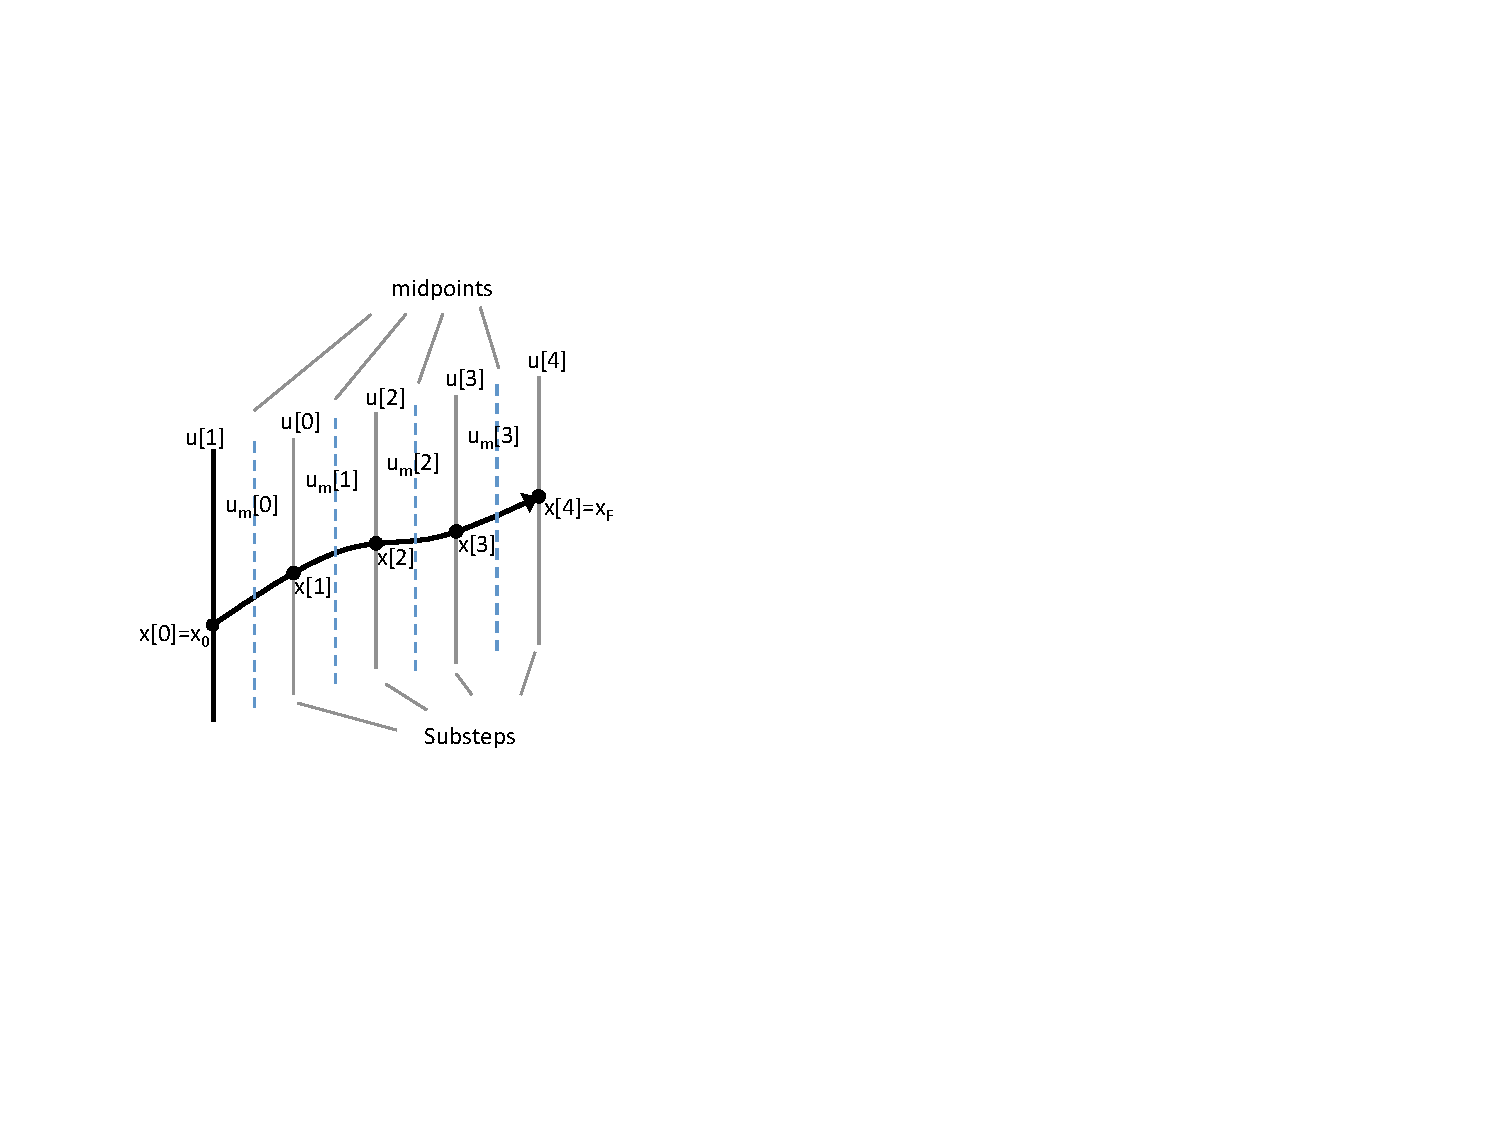
\includegraphics[width=.38\textwidth]{Figures/singleShooting.pdf}
\vspace{-2mm} 
\caption{Time discretization of trajectory. In the particular case illustrated, there are $N=4$ substeps. The initial time $t_0$ corresponds to $n=0$ and the final time of the trajectory corresponds to $n=N$.}
\label{fig:singleShoot}
\end{figure}

To proceed, we must first discretize the trajectory in time for purposes of numerical integration. Following the procedure of~\cite{betts2001practical}, we divide the trajectory into substeps evenly distributed in time and specify the state ($\bs x$) and control ($\bs u$) at each substep. Additionally, we define the value of the control at midpoints, points half way between each substep. For example, see Figure~\ref{fig:singleShoot}, where the trajectory is divided into $N=4$ substeps:  $\bs x[n]_{n = 0, \dots, N}$, $\bs u[n]_{n = 0, \dots, N}$, and $\bs u_M[n]_{n=0,\dots, N-1}$.


\subsection{Explicit Euler Integration}

Consider explicit Euler integration of the dynamics~\eqref{eq:dynamics},
\begin{equation*}
\begin{split}
&\bs x[n+1] = \bs x[n] + dt \bs f(t_n, \bs x[n], \bs u[n]), \quad dt = \frac{t_F-t_0}{N}, \quad t_n = t_0 + n dt.
%&J^{\bs \alpha} = h(t_0,t_F,\bs x[0], \bs x[N]) + \sum_{n=0}^{N-1} dt g(t_n,\bs x[n],\bs u[n])
\end{split}
\end{equation*}
Integrating the cost function~\eqref{eq:Cost} in the same manner, we have
\begin{equation*}
J^{\bs \alpha} = h(t_0,t_F,\bs x[0], \bs x[N]) + \sum_{n=0}^{N-1} dt g(t_n,\bs x[n],\bs u[n]),
\end{equation*}
and the gradient is found be repeatedly carrying out the chain rule,
\begin{equation*}
\begin{split}
\frac{\partial J^{\bs \alpha}}{\partial \bs \alpha} = & 
\frac{\partial h(t_0,t_F,\bs x[0], \bs x[N])}{\partial t_0}\frac{\partial t_0}{\partial \bs \alpha} + 
\frac{\partial h(t_0,t_F,\bs x[0], \bs x[N])}{\partial t_F}\frac{\partial t_F}{\partial \bs \alpha} + 
\frac{\partial h(t_0,t_F,\bs x[0], \bs x[N])}{\partial \bs x[0]}\frac{\partial \bs x[0]}{\partial \bs \alpha} \\
+ & \frac{\partial h(t_0,t_F,\bs x[0], \bs x[N])}{\partial \bs x[N]}\frac{\partial \bs x[N]}{\partial \bs \alpha} +   
\frac{\partial dt}{\partial \bs \alpha}  \sum_{n=0}^{N-1}g(t_n,\bs x[n],\bs u[n])  \\
+ & \sum_{n=0}^{N-1} dt \left ( \frac{\partial g(t_n,\bs x[n],\bs u[n])}{\partial  t_n}\frac{\partial t_n}{\partial \bs \alpha} +
\frac{\partial g(t_n,\bs x[n],\bs u[n])}{\partial \bs x}\frac{\partial \bs x[n]}{\partial \bs \alpha} + 
\frac{\partial g(t_n,\bs x[n],\bs u[n])}{\partial \bs u}\frac{\partial \bs u[n]}{\partial \bs \alpha}   \right)\\
\end{split}
\end{equation*}

The terms $\partial \bs x[n]/\partial \bs \alpha$ can be obtained while integrating the dynamics forward, we have, 
\begin{equation}
\begin{split}
\frac{\partial \bs x[n+1]}{\partial \bs \alpha} &= \frac{\partial \bs x[n]}{\partial \bs \alpha} + {d t} \left( \frac{\partial \bs f(t_n,\bs x[n], \bs u[n])}{\partial t}\frac{\partial t_n}{\partial \bs \alpha} + \frac{\partial \bs f(t_n,\bs x[n], \bs u[n])}{\partial \bs x}\frac{\partial \bs x[n]}{\partial \bs \alpha}  + \frac{\partial \bs f(t_n,\bs x[n], \bs u[n])}{\partial \bs u}\frac{\partial \bs u [n]}{\partial \bs \alpha}\right)  \\
+ & \frac{\partial dt}{\partial \bs \alpha}  \bs f(t_n,\bs x[n],\bs u[n]).
\end{split}
\label{eq:dxda}
\end{equation}

and the remaining terms, $\partial \bs x[0] /\partial\bs \alpha $, $\partial \bs u[n]/\partial \bs \alpha$, $\partial t_0 / \partial \bs \alpha$, etc. depend on the particular definition of $\bs \alpha$ in question. For example, take $\bs \alpha = \bs x_0$, in which case we have
\begin{align*}
\frac{\partial \bs x[0]}{\partial \bs \alpha} = \bs I, \quad  \frac{\partial \bs u[n]}{\partial \bs \alpha} = 0, \quad 
\frac{\partial t_0}{\partial \bs \alpha} =0, \quad \text{etc.}
\end{align*} 
Considering another possibility: $\bs \alpha^T = [t_0, t_F, \bs x_0^T, \bs u_0^T, (\bs u^M_0)^T, \bs u_1^T, (\bs u^M_1)^T ... , \bs u_N^T ]$, i.e. an open-loop control policy, then we have, 
\begin{align*}
\frac{\partial \bs x[0]}{\partial \bs \alpha} = 
\begin{bmatrix}
\bs 0 & \bs 0 & \bs I & \bs 0 & \dots & \bs 0
\end{bmatrix}, \quad  
\frac{\partial \bs u[0]}{\partial \bs \alpha} = 
\begin{bmatrix}
\bs 0 & \bs 0 & \bs 0 & \bs I & \bs 0 & \dots & \bs 0
\end{bmatrix}, \quad 
\frac{\partial t_0}{\partial \bs \alpha} =
\begin{bmatrix}
1 & 0 & \dots & 0 
\end{bmatrix}
, \quad \text{etc.}
\end{align*} 
Note, for the explicit Euler integration scheme, the midpoint control values were not involved, but they are involved in the 4$^{\text{th}}$ order Runge-Kutta scheme below.


\section{Multiple-Shooting Formulation}
So far we have only considered the single shooting approach. In the multiple shooting approach, the trajectory is divided into multiple segments as shown in Figure~\ref{fig:multShoot}. Discrepancies between the endpoints of the segments are accounted for by defect constraints. If the trajectory is divided into $N_S$ segments, this requires the introduction of the optimization parameters $\bs x_1$, $\bs x_2$, $\dots$, $\bs x_{N_S-1}$. Now, the terms $\partial \bs x[n]/\partial \bs \alpha$ can be calculated separately for each shooting segment to determine gradients of the cost function and any constraint functions. For example, consider the first defect constraint of Figure~\ref{fig:multShoot},
\begin{equation*}
\bs\Delta_0 = \bs x_0^{+} - \bs x_1.
\end{equation*}
and take the set of optimization parameters to be 
\begin{equation*}
\bs \alpha = \lbrack t_0, t_F, \bs x_0^T, \bs x_1^T, \bs x_2^T, \bs x_{F}^T, \bs u_0^T, (\bs u^M_0)^T, \bs u_1^T, (\bs u^M_1)^T, \dots , \bs u_N^T \rbrack.
\end{equation*}
The gradient, $\partial \bs\Delta_0/\partial \bs\alpha$, requires $\partial\bs x_0^{+}/\partial \bs \alpha$ and $\partial\bs x_1/\partial \bs \alpha$. The first term can be obtained by carrying out the recursive equation~\eqref{eq:dxda}, over the first shooting segment starting from 
\begin{equation}
\frac{\partial \bs x[0]}{\partial \bs \alpha} = 
\frac{\partial \bs x_0}{\partial \bs \alpha} =
\begin{bmatrix}
\bs 0 & \bs 0 & \bs I & \bs 0 & \dots & \bs 0
\end{bmatrix}.
\end{equation}
Similarly, to determine the gradient of second defect, the term $\partial\bs x_0^{+}/\partial \bs \alpha$ is evaluated using~\eqref{eq:dxda} over the second segment starting from 
\begin{equation}
\frac{\partial \bs x[2]}{\partial \bs \alpha} = 
\frac{\partial \bs x_1}{\partial \bs \alpha} =
\begin{bmatrix}
\bs 0 & \bs 0 & \bs 0 & \bs I & \dots & \bs 0
\end{bmatrix}.
\end{equation}

%\begin{figure}[h]
%\centering
%\hspace{0mm}
%\includegraphics[width=.47\textwidth]{Figures/multipleShooting_Defects.pdf}
%\vspace{-3mm} 
%\caption{Multiple shooting case. The trajectory is divided into segments. In this particular case $N_S=3$ segments.}
%\label{fig:multShootDefects}
%\end{figure}

\begin{figure}[h]
\centering
\hspace{0mm}
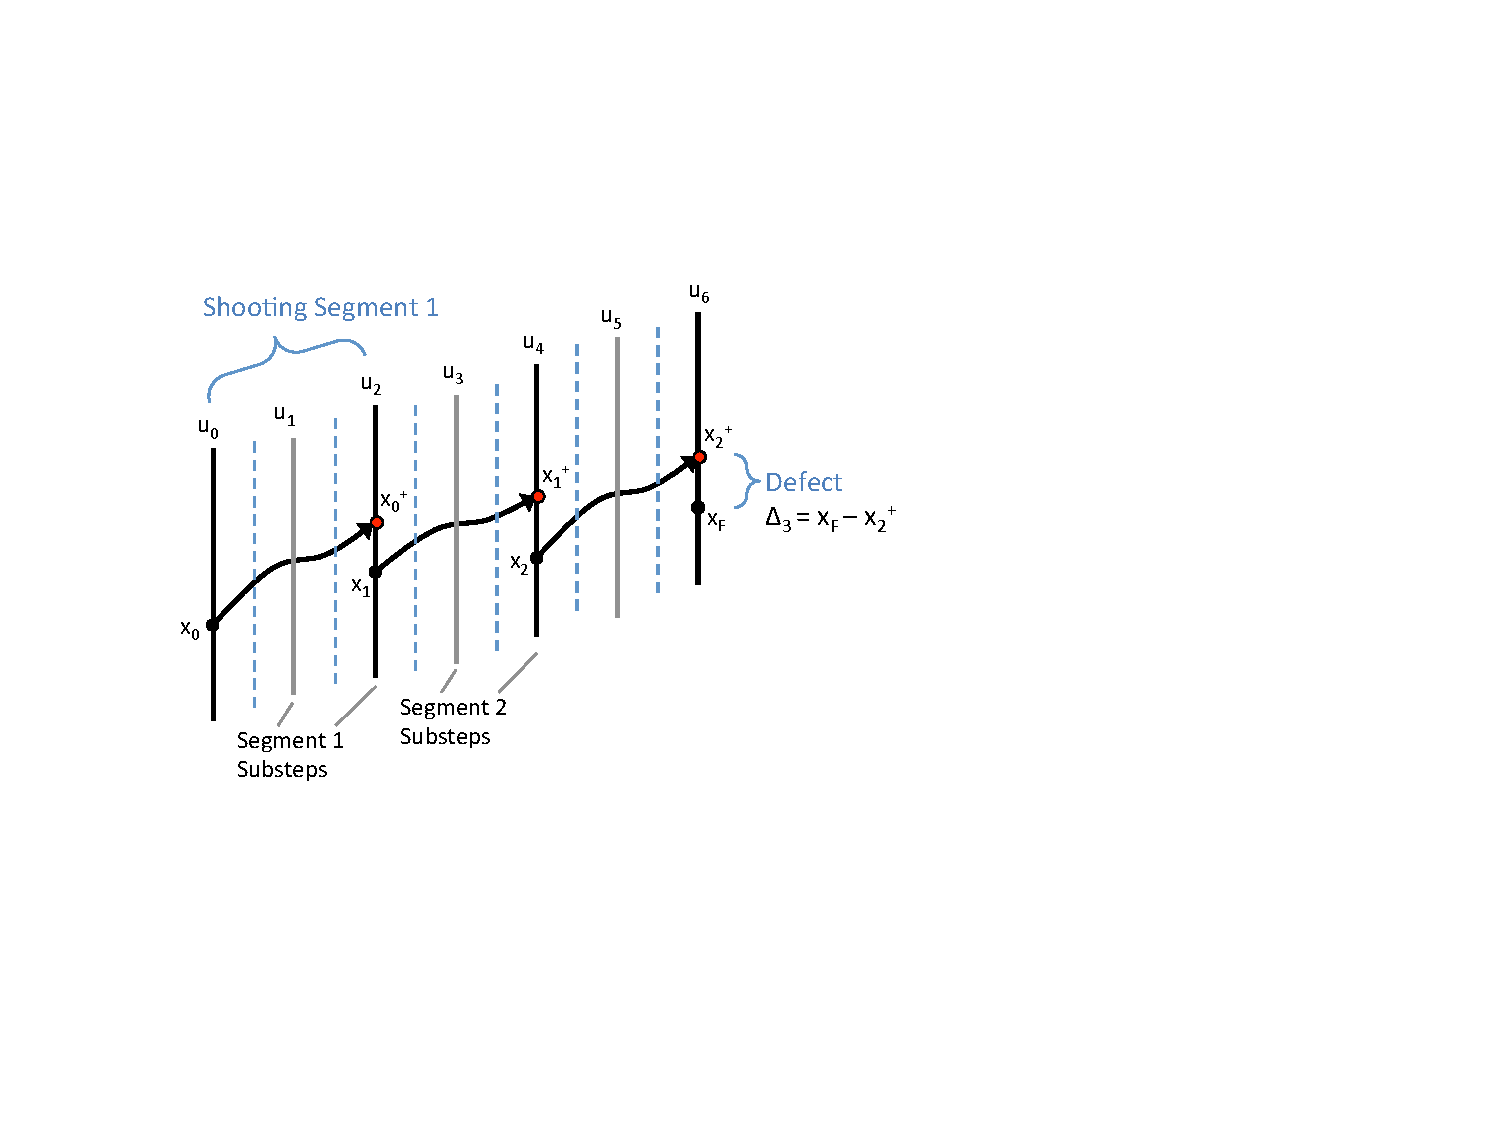
\includegraphics[width=.5\textwidth]{Figures/multipleShooting.pdf}
\vspace{-3mm} 
\caption{Multiple shooting case. The trajectory is divided into segments. In this particular case $N_S=3$ segments and $N=2$ substeps for each segment.}
\label{fig:multShoot}
\end{figure}


\section{Other Integration Schemes}

\subsection{4$^{\text{th}}$ Order Runge-Kutta Integration}
See the function \texttt{simSysGrad} inside \texttt{rungeKutta.m} of the OptimTraj package for the matlab implementation of the following equations. Consider the path cost 
\begin{equation}
J^{\bs \alpha} = \int_{t_0}^{t_F}  g(t, \bs x(t), \bs u(t)) dt,
\label{eq:PathCost}
\end{equation}
and employ a 4th-order Runge-Kutta scheme for integration of the dynamics and cost function, 
\begin{align*}
J^{\bs\alpha} = & \sum_{n=0}^{N-1} \frac{dt}{6} \left(  g_0[n] +  g_1[n] +  g_2[n] +  g_3[n]\right)   &\quad \bs x[n+1] &= \bs x[n] + \frac{dt}{6} \left(\bs k_0[n] + \bs k_1[n] + \bs k_2[n] + \bs k_3[n]\right)\\
g_0[n] &=  g(t_n, \bs x[n], \bs u[n])  &\bs k_0[n] & = \bs f(t_n, \bs x[n], \bs u[n])\\
g_1[n] &=  g(t_n + 0.5dt, \bs x[n] + 0.5dt\; \bs k_0, \bs u^M[n]) &\bs k_1[n] & = \bs f(t_n + 0.5dt, \bs x[n] + 0.5dt\; \bs k_0, \bs u^M[n])\\
g_2[n] &=  g(t_n+0.5dt, \bs x[n] + 0.5dt\; \bs k_1, \bs u^M[n]) &\bs k_2[n] & = \bs f(t_n+0.5dt, \bs x[n] + 0.5dt\; \bs k_1, \bs u^M[n])\\
g_3[n] &=  g(t_n+dt, \bs x[n] + dt\; \bs k_2, \bs u[n+1]) &\bs k_3[n] & = \bs f(t_n+dt, \bs x[n] + dt\; \bs k_2, \bs u[n+1])
\end{align*}
The gradient of the cost function w.r.t. the decision parameter $\bs \alpha$ is 
\begin{equation*}
\frac{\partial J}{\partial \bs \alpha} = \sum_{n=0}^{N-1}\frac{d t}{6} \left(\frac{\partial g_0[n]}{\partial \bs \alpha} + \frac{\partial g_1[n]}{\partial \bs \alpha} + \frac{\partial g_2[n]}{\partial \bs \alpha} + \frac{\partial g_3[n]}{\partial \bs \alpha}  \right) + \frac{1}{6}\frac{\partial dt}{\partial \bs\alpha} \left(g_0[n] + g_1[n] + g_2[n] + g_3[n]\right)
\end{equation*}
where 
\begin{equation*}
\begin{split}
\frac{\partial \bs x[n+1]}{\partial \bs \alpha} &= \frac{\partial \bs x[n]}{\partial \bs \alpha} + \frac{d t}{6} \left(\frac{\partial \bs k_0[n]}{\partial \bs \alpha} + \frac{\partial \bs k_1[n]}{\partial \bs \alpha} + \frac{\partial \bs k_2[n]}{\partial \bs \alpha} + \frac{\partial \bs k_3[n]}{\partial \bs \alpha}  \right) + \frac{1}{6}\frac{\partial dt}{\partial \bs\alpha} \left(\bs k_0[n] + \bs k_1[n] + \bs k_2[n] + \bs k_3[n]\right)
\end{split}
\end{equation*}
Now, all that's left is to obtain the terms, $  {\partial \bs k_i[n]}/{\partial \bs \alpha}$ and $  {\partial g_i[n]}/{\partial \bs \alpha}$ . This is where things start to get a bit ugly, but, again, it's just a repeated carrying out of the chain rule,
\begin{equation*}
\begin{split}
\frac{\partial \bs k_0}{\partial \bs \alpha} =& \frac{\partial \bs f(t_n,\bs x[n], \bs u[n])}{\partial t}\frac{\partial t_n}{\partial \bs \alpha} + \frac{\partial \bs f(t_n,\bs x[n], \bs u[n])}{\partial \bs x}\frac{\partial \bs x[n]}{\partial \bs \alpha}  + \frac{\partial \bs f(t_n,\bs x[n], \bs u[n])}{\partial \bs u}\frac{\partial \bs u [n]}{\partial \bs \alpha},
\\[2ex]
\frac{\partial \bs k_1}{\partial \bs \alpha} =& \frac{\partial \bs f(t_n+0.5dt,\bs x[n]+0.5dt \bs k_0,\bs u^M[n])}{\partial t} \left( \frac{\partial t_n}{\partial \bs \alpha} + 0.5\frac{\partial dt}{\partial \bs \alpha}  \right)+\\
& \frac{\partial \bs f(t_n+0.5dt,\bs x[n]+0.5dt \bs k_0,\bs u^M[n])}{\partial \bs x} \left( \frac{\partial \bs x[n]}{\partial \bs \alpha} + 0.5\bs k_0\frac{\partial dt}{\partial \bs \alpha} + 0.5dt\frac{\partial \bs k_0}{\partial \bs \alpha}  \right) +\\
&  \frac{\partial \bs f(t_n+0.5dt,\bs x[n]+0.5dt \bs k_0,\bs u^M[n])}{\partial \bs u}\frac{\partial \bs u^M[n]}{\partial \bs \alpha},
\\
\end{split}
\end{equation*}
\begin{equation*}
\begin{split}
\frac{\partial \bs k_2}{\partial \bs \alpha} =& \frac{\partial \bs f(t_n+0.5dt,\bs x[n]+0.5dt \bs k_1,\bs u^M[n])}{\partial t} \left( \frac{\partial t_n}{\partial \bs \alpha} + 0.5\frac{\partial dt}{\partial \bs \alpha}  \right)+\\
& \frac{\partial \bs f(t_n+0.5dt,\bs x[n]+0.5dt \bs k_1,\bs u^M[n])}{\partial \bs x} \left( \frac{\partial \bs x[n]}{\partial \bs \alpha} + 0.5\bs k_1\frac{\partial dt}{\partial \bs \alpha} + 0.5dt\frac{\partial \bs k_1}{\partial \bs \alpha}  \right) +\\
&  \frac{\partial \bs f(t_n+0.5dt,\bs x[n]+0.5dt \bs k_1,\bs u^M[n])}{\partial \bs u}\frac{\partial \bs u^M[n]}{\partial \bs \alpha},
\\[2ex]
\frac{\partial \bs k_3}{\partial \bs \alpha} =& \frac{\partial \bs f(t_n+dt,\bs x[n]+dt \bs k_2,\bs u[n+1])}{\partial t} \left( \frac{\partial t_n}{\partial \bs \alpha} + \frac{\partial dt}{\partial \bs \alpha}  \right)+\\
& \frac{\partial \bs f(t_n+dt,\bs x[n]+dt \bs k_2,\bs u[n+1])}{\partial \bs x} \left( \frac{\partial \bs x[n]}{\partial \bs \alpha} + \bs k_2\frac{\partial dt}{\partial \bs \alpha} + dt\frac{\partial \bs k_2}{\partial \bs \alpha}  \right) +\\
&  \frac{\partial \bs f(t_n+dt,\bs x[n]+dt \bs k_2,\bs u[n+1])}{\partial \bs u}\frac{\partial \bs u[n+1]}{\partial \bs \alpha},
\\[1ex]
\end{split}
\end{equation*}
The terms $  {\partial g_i[n]}/{\partial \bs \alpha}$ are very similar to $  {\partial \bs k_i[n]}/{\partial \bs \alpha}$. In each instance, simply replace $\bs k_i$ with $g_i$ and $\bs f$ with $g$ to obtain $  {\partial g_i[n]}/{\partial \bs \alpha}$.


\bibliographystyle{IEEEtran}
\bibliography{biblio}    
\end{document}
